\documentclass[a4paper,12pt]{article}
\usepackage{amsmath}
\usepackage{amssymb}
\usepackage[polish]{babel}
\usepackage{polski}
\usepackage[utf8]{inputenc}
\usepackage{indentfirst}
\usepackage{geometry}
\usepackage{array}
\usepackage[pdftex]{color,graphicx}
\usepackage{subfigure}
\usepackage{afterpage}
\usepackage{setspace}
\usepackage{color}
\usepackage{wrapfig}
\usepackage{listings}
\usepackage{datetime}

\renewcommand{\onehalfspacing}{\setstretch{1.6}}

\geometry{tmargin=2.5cm,bmargin=2.5cm,lmargin=2.5cm,rmargin=2.5cm}
\setlength{\parindent}{1cm}
\setlength{\parskip}{0mm}

\newenvironment{lista}{
\begin{itemize}
  \setlength{\itemsep}{1pt}
  \setlength{\parskip}{0pt}
  \setlength{\parsep}{0pt}
}{\end{itemize}}

\newcommand{\linia}{\rule{\linewidth}{0.4mm}}

\definecolor{lbcolor}{rgb}{0.95,0.95,0.95}
\lstset{
    backgroundcolor=\color{lbcolor},
    tabsize=4,
  language=C++,
  captionpos=b,
  tabsize=3,
  frame=lines,
  numbers=left,
  numberstyle=\tiny,
  numbersep=5pt,
  breaklines=true,
  showstringspaces=false,
  basicstyle=\footnotesize,
  identifierstyle=\color{magenta},
  keywordstyle=\color[rgb]{0,0,1},
  commentstyle=\color{Darkgreen},
  stringstyle=\color{red}
  }

\begin{document}

\noindent
\begin{tabular}{|c|p{11cm}|c|} \hline 
Grupa 4 & Katarzyna Kosiak i Michał Folwarski & \ddmmyyyydate\today \tabularnewline
\hline 
\end{tabular}


\section*{Zadanie 1 - Filtr Gaussa i OpenMP}

Program rozmywa zadane zdjęcie za pomocą algorytmu Gaussa z maską o wymiarach 5x5 korzystając z zadanej liczby wątków.
Zrównoleglono rozmywanie rzędów pikseli zadanego zdjęcia: 
\begin{lstlisting}
#pragma omp parallel for num_threads(numberOfThreads) default(shared) private(i,j)
    for (i=0; i < rows; i++) {
        for (j = 0; j < cols; j++) {
            /obliczanie nowych wartosci R,G i B dla piksela
        }
    }
\end{lstlisting}
Zastosowano takie instrukcje OpenMP ponieważ:
\begin{lista}
 \item for: zrównoleglamy pętlę for (przebieg po wierszach),
 \item num threads: zrównoleglanie na zadaną w argumentach wywołania programu liczbę wątków,
 \item default(shared): dla wygody domyślnie każda zmienna jest dostępna dla każdego wątku,
 \item private(i,j): każdy wątek dostaje kopię zmiennych przechowujących indeksy aktualnej iteracji.
\end{lista}

Domyślnie OpenMP rozdzieli pracę nad pętlą równomiernie pomiędzy wszystkie wątki. Ponieważ rozmywanie każdego piksela opiera się na tych samych działaniach (kolejne piksele nie stają się trudniejsze dto przetworzenia) to taki podział nam odpowiada.\\

Zalety tego rozwiązania to: 
\begin{lista}
 \item Dobrze zrównolegla obliczenia przy zachowaniu prostoty konfiguracji,
 \item Nie wymaga dodatkowych zasobów poza dostępnymi procesorami.
\end{lista}


Umieszczony poniżej wykres (Rysunek 1) pokazuje zależność czasu działania programu od liczby wątków dla przykładowego obrazu o rozmiarze boku około 2500px na komputerze z dwoma procesorami. \\
Jak widać czas skrócił się przy zrównolegleniu na tyle wątków, ile jest procesorów. Dalsze zwiększanie liczby wątków może tylko pogorszyć czas, ponieważ musi zostać poświęcony dodatkowy czas na przełączanie konktekstu dla poszczególnych wątków na współdzielonych procesorach.
\begin{figure}[h]
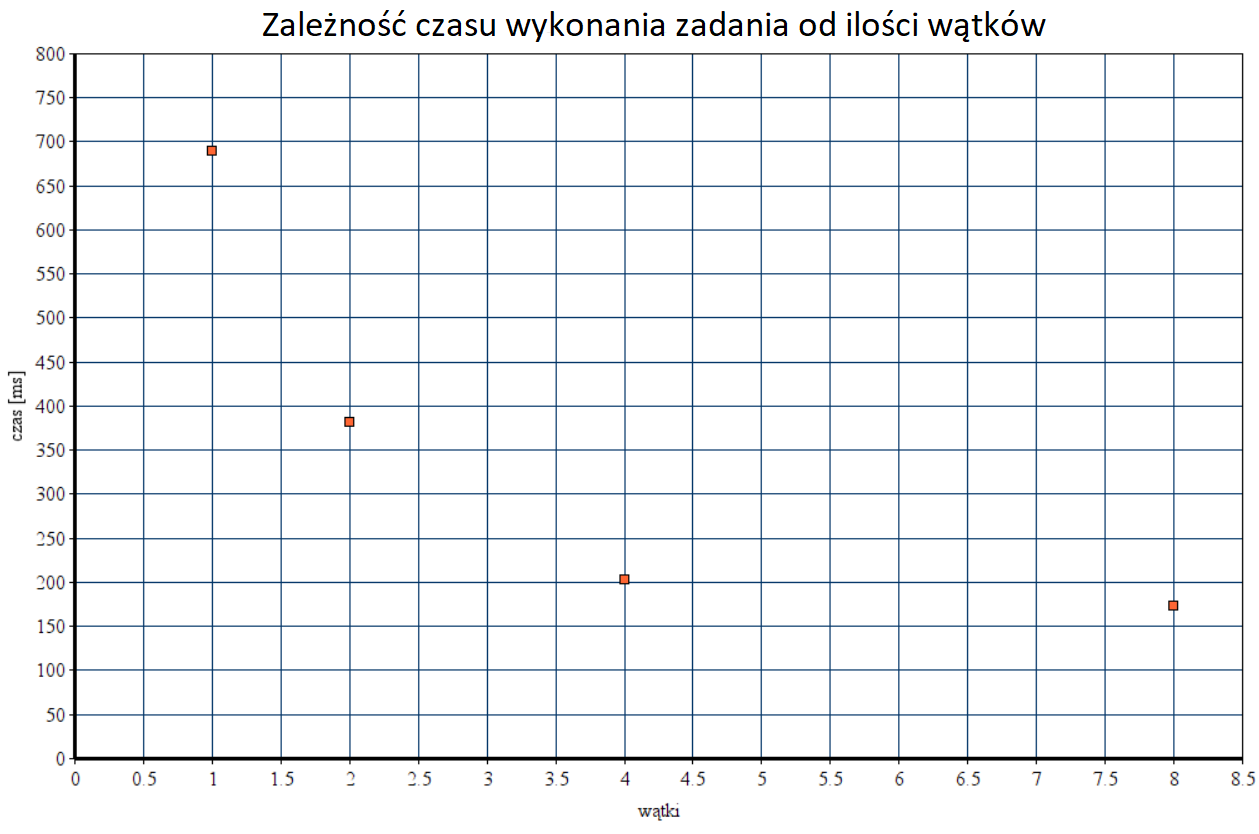
\includegraphics[width=15cm]{wykres_zad1}
\caption{}  
\end{figure}
\\

Wnioski \\
Zadanie udało się wykonać - dokonano zrównoleglenia obliczeń. Wykorzystanie OpenMP w tym przypadku (niezależne od siebie obliczenia o tej samej złożoności) było skuteczne i nie wymagało wiele konfiguracji. 
\end{document}
